\chapter{Anatomia e fisiopatologia renale}
 
\begin{flushright}
\textit{``La fixité du milieu intérieur est la condition \\de la vie libre et indépendante''}
\end{flushright}
\begin{flushright} \textsc{Claude Bernard} (1813 - 1878) \end{flushright}
\begin{flushright} { } \end{flushright}
Claude Bernard, fisiologo francese, riuscì a mostrare che la medicina basata su esperimenti e fatti era superiore a quella basata su teorie e precedenti storici. Fece capire, inoltre, come per conseguire tale obiettivo i medici avessero bisogno di una esperienza molto più profonda di ciò che accade nel corpo, non soltanto nel corpo sano ma anche in quello malato. Uno dei concetti più importanti che introdusse fu quello del \textit{milieu interiéur} e notò che <<tutti i meccanismi vitali, per quanto possano essere differenti, hanno un unico scopo: quello di mantenere costanti le condizioni vitali nel sistema interno>>\footnote{H. Hellman, ``\textit{Le dispute della medicina. Dieci casi esemplari}'' Raffaello Cortina Editore.}.
Questa teoria ha avuto enormi conseguenze. Nel 1926 indusse Walter Cannon, fisiologo di Harvard, a sviluppare il concetto di \textit{omeostasi}, cioè dell'insieme di diversi processi fisiologici atti a conservare il nostro corpo in equilibrio, nonstante le fluttuazioni delle condizioni ambientali. La stessa idea doveva portare, più tardi, alla formulazione della nozione di \textit{feedback} da parte del matematico, e padre della cibernetica\footnote{dal greco $\kappa\upsilon\beta\varepsilon\rho\nu\acute{\eta}\tau\eta\varsigma$ (timoniere). Wiener coniò il termine \textit{cibernetica} per descrivere l'applicazione della ``teoria del controllo'' alla fisiologia, anche se, al giorno d'oggi, il termine è spesso associato alla robotica.}, Norbert Wiener \cite{khoo}.

L'omeostasi del \textit{milieu interieur}, compresi il volume, la composizione e la distribuzione dei fluidi corporei, è quindi essenziale per la sopravvivenza. Per bilanciare l'assorbimento quotidiano di cibo e acqua, e mantenere l'omeostasi, sono necessari meccanismi di escrezione controllati finemente. Parallelamente ai contributi di intestino, polmoni e cute, la funzione di controllo sulla quantità e composizione di fluidi e soluti è svolta dai reni.

\section{Anatomia del rene}
I due reni giacciono sulla parete posteriore dell'addome, all'esterno della cavità peritoneale (\figurename~\ref{anathomy1}). Ciascun rene presenta, nella parte mediana, una rientranza detta \textit{ilo}. Dall'ilo entrano e fuoriescono: arteria e vena renali, i vasi linfatici, i nervi e l'uretere. Quest'ultimo convoglia l'urina prodotta dal rene verso la vescica, dalla quale è espulsa successivamente allo stimolo della minzione. Per una descrizione anatomica più dettagliata si consulti Guyton et al. \cite{guyton}.

Il flusso sanguigno in ingresso ai reni ammonta a circa un quarto della gittata cardiaca, nonostante per garantire la funzionalità non occorra ad essi più di un decimo dell' ossigeno totale in circolo nell'organismo \cite{burton}. La perfusione è quindi di gran lunga sovradimensionata rispetto alle esigenze metaboliche locali, e ciò si riconduce alla funzione filtrante che i reni svolgono. La maggior parte del flusso ematico renale è infatti convogliato verso i nefroni, che sono le unità funzionali attraverso cui il sangue è continuamente filtrato e purificato.
\begin{figure}[htb]
	\centering
		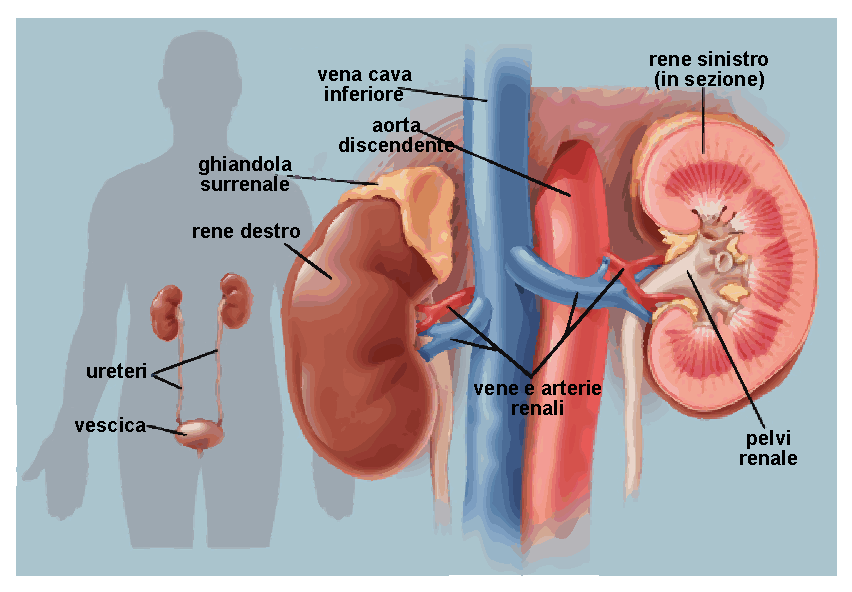
\includegraphics[width=0.9\textwidth]{immagini/anathomy1.eps}
		\caption{Localizzazione anatomica dei reni.}\label{anathomy1}
\end{figure}

\subsection{Il Nefrone \cite{guyton}}
Ogni rene è costituito da circa un milione di nefroni. La \figurename~\ref{anatomia} mostra in dettaglio il nefrone, che è composto da due strutture principali: 
\begin{itemize}
	\item il \textbf{glomerulo}, cioè un groviglio di capillari in cui il sangue è filtrato sotto la spinta della pressione arteriosa;
	\item il \textbf{tubulo renale}, nel quale il filtrato glomerulare è in parte riassorbito e in parte convogliato verso gli ureteri.
\end{itemize}

\begin{figure}[p]
	\centering
	\advance\leftskip-.1\textwidth
		\includegraphics[width=1.2\textwidth]{immagini/anatomia.eps}
		\caption{Dettagli anatomici del rene.}\label{anatomia}
\end{figure}

Il glomerulo è costituito da una fitta rete di capillari ramificati e rivestiti da cellule epiteliali; l'involucro che avvolge il il glomerulo si chiama \textit{capsula di Bowman}. Il liquido filtrato dai capillari glomerulari è raccolto nella capsula di Bowman e convogliato nel \textit{tubulo prossimale}, localizzato nella parte corticale del rene. Dal tubulo prossimale il liquido passa nell'\textit{ansa di Henle}, situata nella zona midollare, in cui avviene il riassorbimento di sostanze utili e la secrezione di cataboliti da e verso il lume dell'ansa. Con un tratto ascendente il percorso del filtrato prosegue verso la \textit{macula densa}, che ha un ruolo di \textit{feedback} molto importante per la modulazione della capacità filtrante del nefrone. Dopo la macula densa il liquido giunge, attraverso una serie di dotti collettori, nel \textit{bacinetto renale} e di li, attraverso gli \textit{ureteri}, nella vescica, dalla quale è espulso per minzione.

\section{Fisiologia renale}
L'eliminazione continua dal plasma dei fluidi in eccesso e di tutte le impurità, contribuendo all'omeostasi dell'organismo, è solo una delle funzioni dei reni. I reni intervengono anche nella regolazione ormonale dei processi metabolici, perché sono anche dotati di un sistema endocrino. Un esempio è la capacità di controllo della pressione arteriosa attraverso la liberazione seriale di ormoni che agiscono direttamente sullo stato vasopressivo del circuito arterioso (sistema \textit{renina-angiotestina-aldosterone}). In sintesi, le funzioni principali svolte dal rene sono:
\begin{itemize}
	\item eliminazione dei cataboliti e riassorbimento di sostanze utili;
	\item regolazione dell'osmolarità e della volemia dei liquidi corporei;
	\item controllo del bilancio elettrolitico e dell'equilibrio acido-base;
	\item regolazione della pressione arteriosa.
\end{itemize}
Nei prossimi paragrafi si illustreranno a grandi linee gli stati di malattia del rene e le possibili terapie.

\section{Patologie renali}
\begin{wrapfigure}{o}{0.4\textwidth}
	\centering
	\vspace{-10pt}
		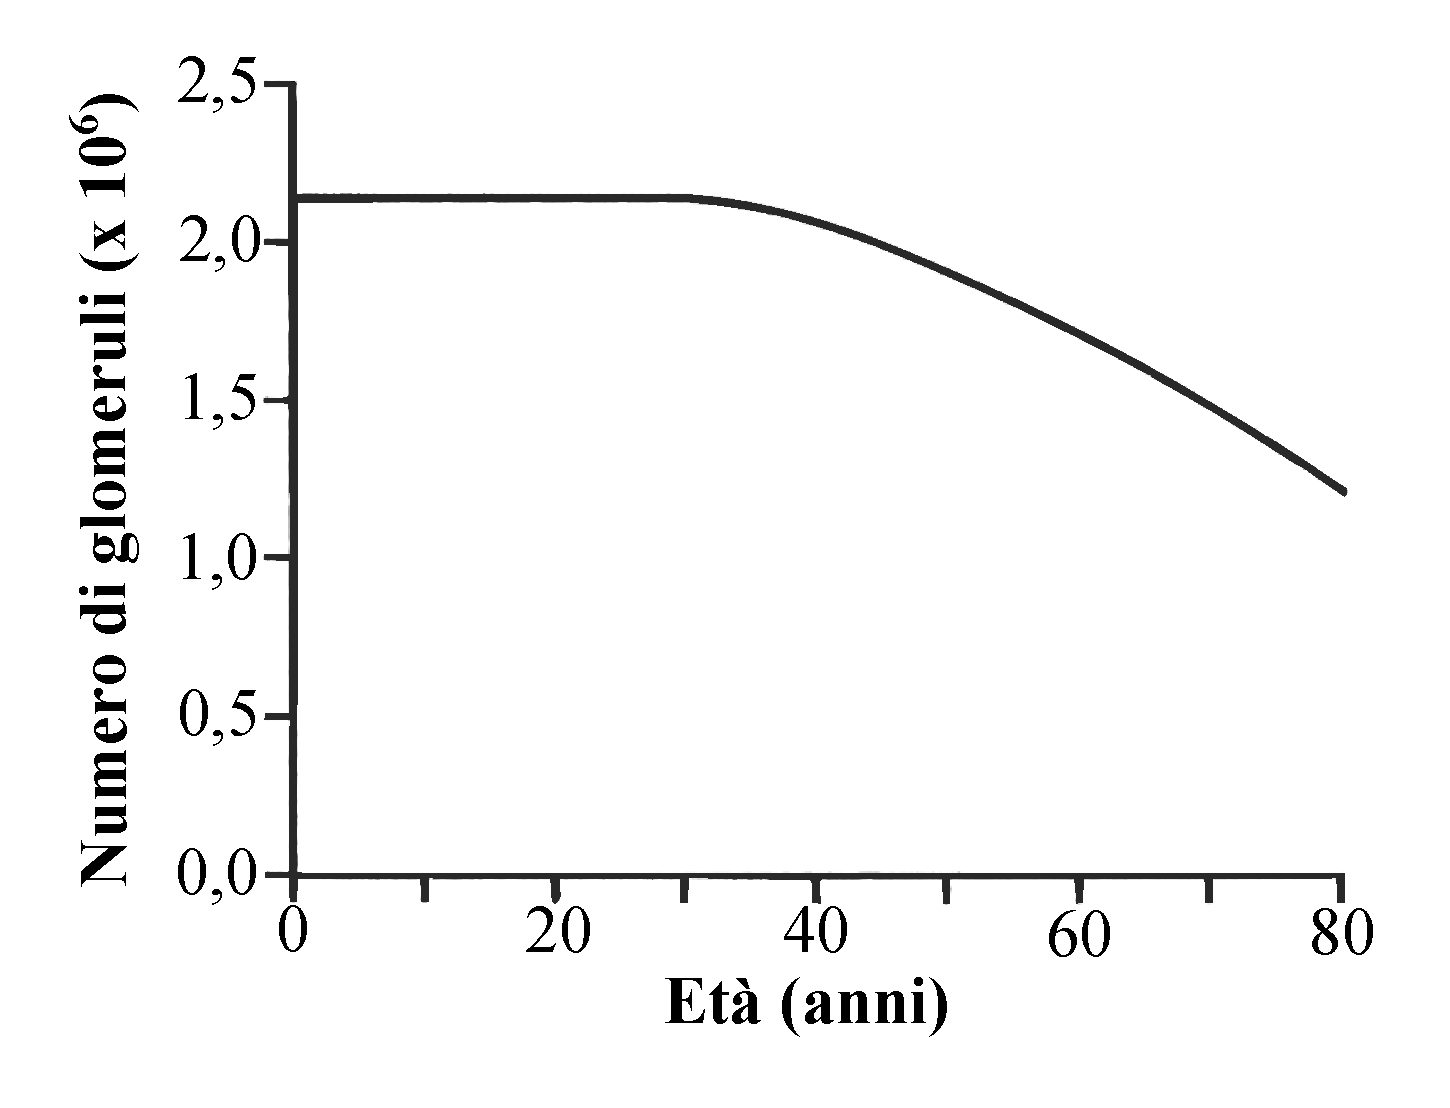
\includegraphics[width=0.4\textwidth]{immagini/eta_gfr.eps}
		\vspace{-20pt}
		\caption{}\label{eta_gfr}
		\vspace{-10pt}
\end{wrapfigure}
L'eziologia delle patologie renali è molto varia e può essere genetica, infettiva, traumatica, vascolare, immunologica, batteriologica o degenerativa \cite{bronzino}.
In un soggetto sano, come mostrato nella \figurename~\ref{eta_gfr}, la performance renale diminuisce gradualmente a partire dai 40 anni fino a dimezzarsi intorno agli 80 anni, senza tuttavia risultare invalidante. Nei casi patologici, quando la funzionalità renale si riduce al $20$-$25\%$ di quella normale, la sopravvivenza dell'individuo è vincolata alla qualità della terapia dialitica cui deve periodicamente sottoporsi.
Le patologie renali possono essere riferite a due categorie generali \cite{guyton}, che sono:
\begin{itemize}
	\item l'insufficienza renale \textbf{acuta}, in cui i reni cessano all'improvviso di funzionare completamente o quasi, ma possono eventualmente recuperare la funzionalità normale;
	\item l'insufficienza renale \textbf{cronica}, nella quale un numero crescente di nefroni perde progressivamente le proprie funzioni, con conseguente degenerazione della funzionalità renale.
\end{itemize}

\subsection{Insufficienza renale acuta \cite{guyton}}
In base alla sede della disfunzione, l'insufficienza renale acuta può essere di tipo:
\begin{itemize}
	\item \textit{\textbf{pre-renale}}, quando l'alterazione si verifica a monte del rene; la sindrome prerenale può verificarsi a seguito di insufficienza cardiaca o a diminuzione del volume del sangue associata a un brusco calo della pressione arteriosa, come nel caso di una grave emorragia;
	\item \textit{\textbf{intra-renale}}, quando le alterazioni sono interne al rene stesso e riguardano i vasi, i glomeruli o i tubuli renali; questa tipologia di disfunzione è solitamente irreversibile e nei casi più gravi sono necessarie cure dialitiche;
	\item \textit{\textbf{post-renale}}, che comporta l'ostruzione del sistema di raccolta dell'urina in qualunque punto, dai calici agli ureteri alle vie di uscita della vescica; le cause principali di ostruzione delle vie urinarie sono i calcoli renali, facilmente eliminabili con tecniche di litotrizione a ultrasuoni o, nei casi più gravi, con la chirurgia.
\end{itemize}
In presenza di insufficienza renale acuta, l'immediato effetto fisiologico è la ritenzione nel sangue e nell'interstizio di acqua, elettroliti e prodotti di scarto del metabolismo, con conseguente ipertensione e edema. In più, l'eccessiva ritenzione di potassio causa aritmie compromettendo la funzionalià cardiaca. Nei casi gravi di insufficienza renale acuta si ha totale anuria che, se non corretta con la dialisi, conduce rapidamente al decesso.

\subsection{Insufficienza renale cronica \cite{guyton}}
Quando la funzionalità renale si riduce fino al $20-25\%$ di quella normale, le lesioni che i nefroni superstiti  subiscono portano a un'ulteriore riduzione della funzionalità renale e, quindi, a un lento circolo vizioso progressivo che si conclude con lo stadio terminale della patologia renale (\figurename~\ref{gfr}). Può quindi accadere che un danno iniziale al rene ne comporti il progressivo deterioramento fino al punto in cui il soggetto, per sopravvivere, deve essere sottoposto a dialisi o a trapianto di rene.
\begin{figure}[htb]
	\centering
		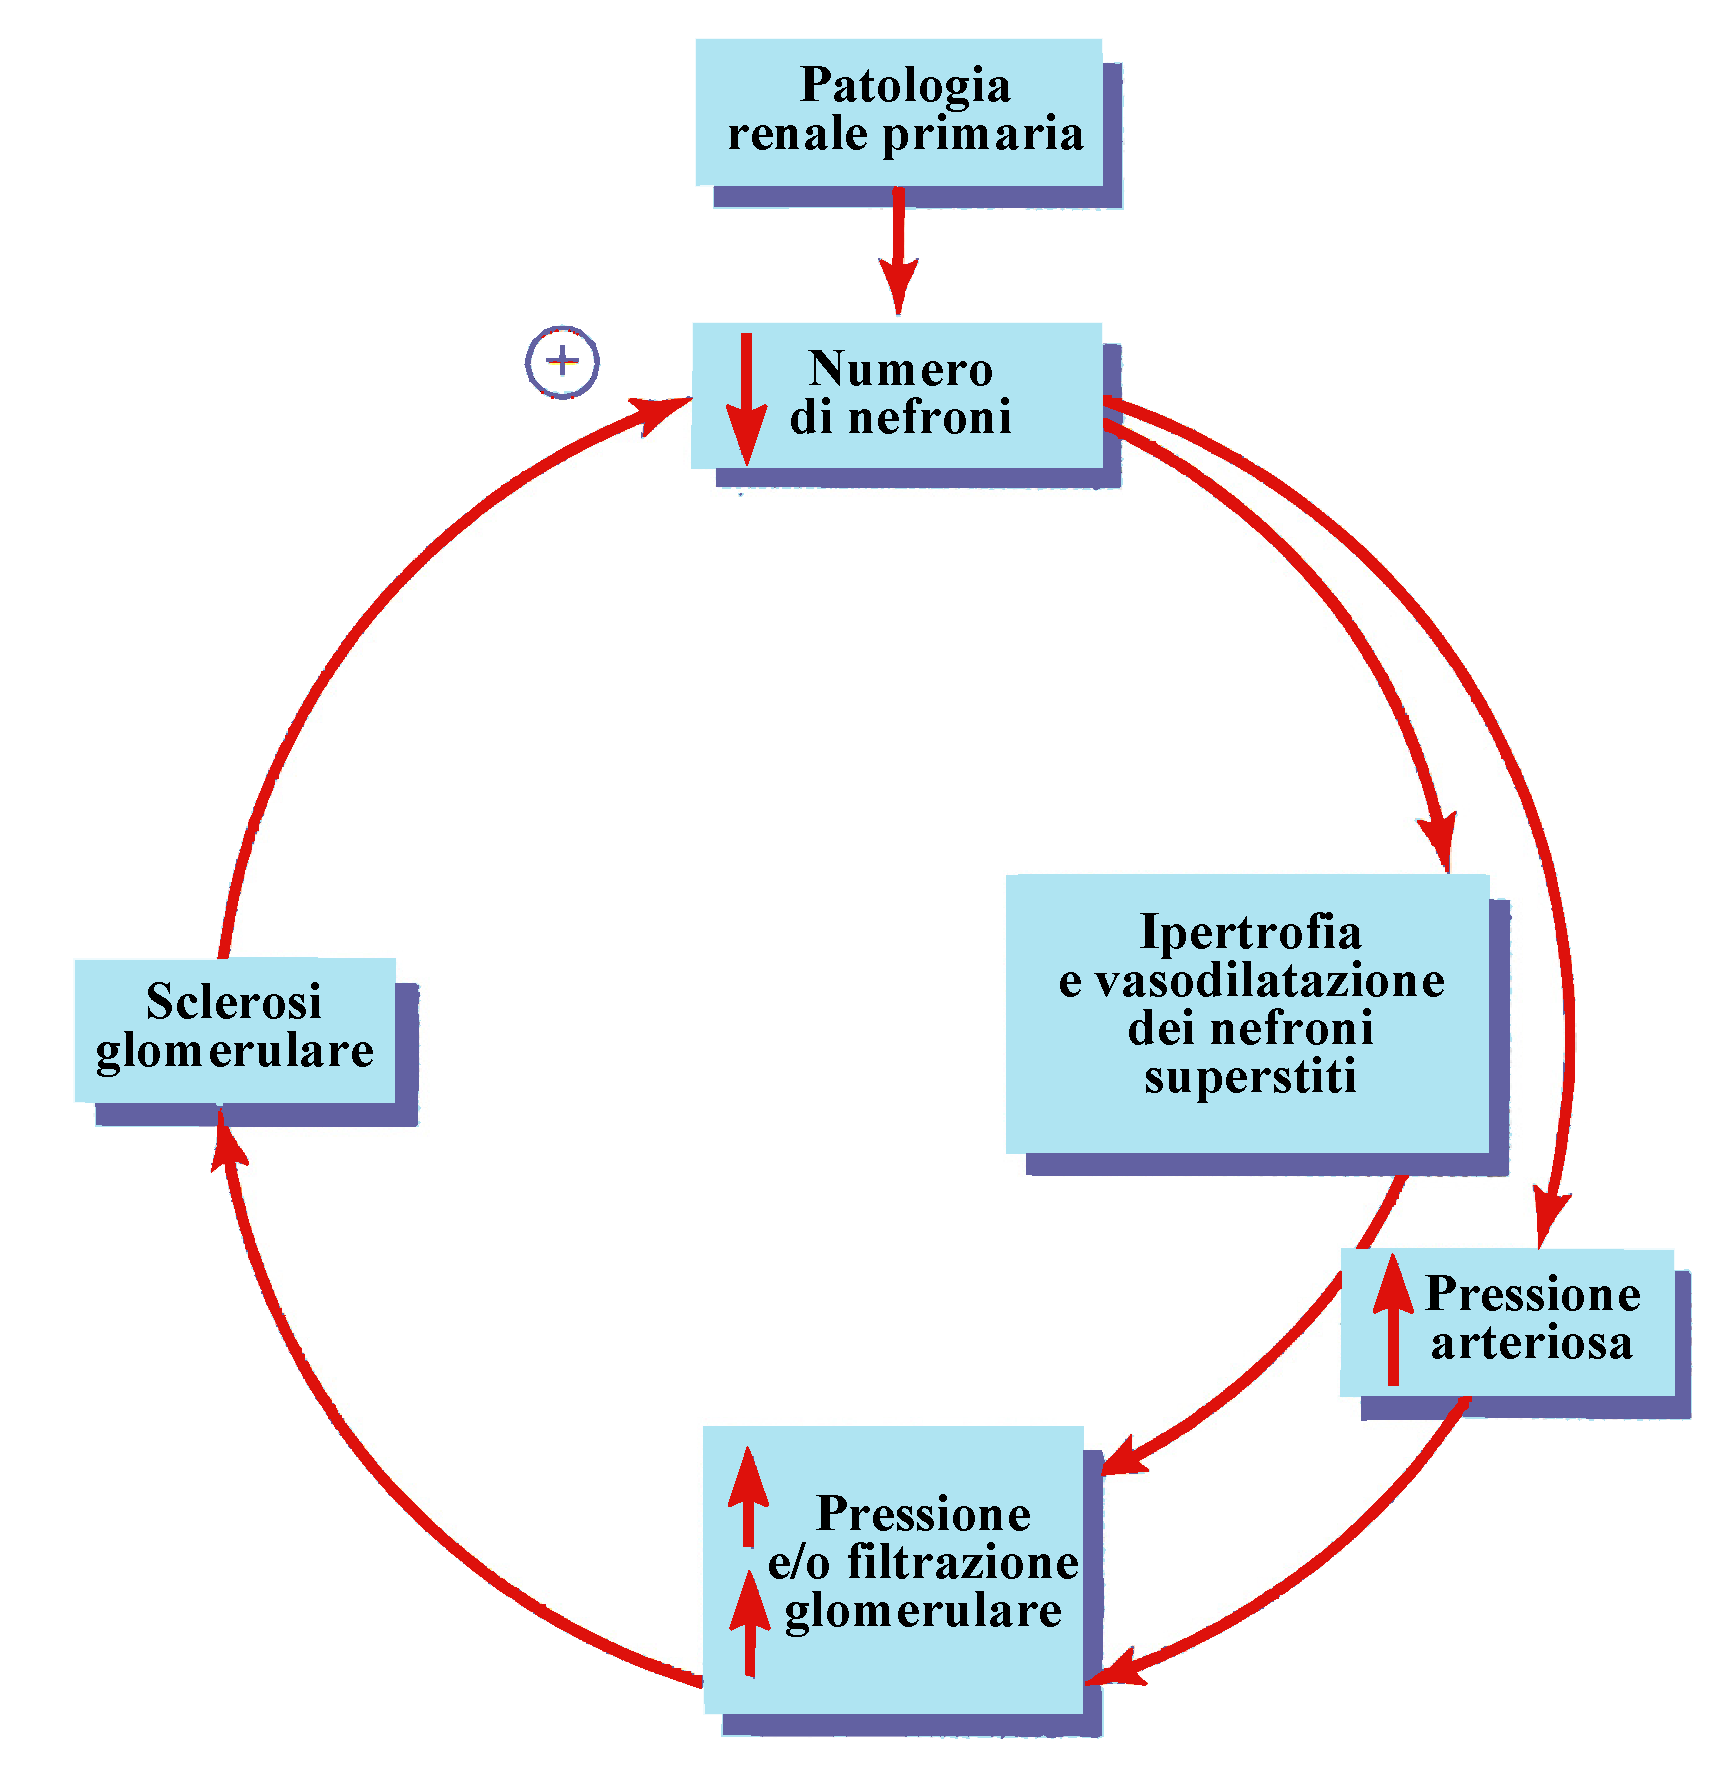
\includegraphics[width=0.7\textwidth]{immagini/gfr.eps}
		\caption{Circolo vizioso che può instaurarsi per una patologia renale primaria. La perdita di nefroni causati dalla patologia può aumentare il flusso e la pressione nei capillari glomerulari restanti; ciò a sua volta può danneggiare anche i capillari sani, causando la loro sclerosi progressiva e alla fine la loro perdita. (Guyton et al. \cite{guyton})}\label{gfr}
\end{figure}


\input capitoli/sections/sec_terapie.tex